\section{Introduction}
\subsection{Introduction to cloud computing and fog computing}
Nowadays we live in a world of data, we create a lot of data per day and we have the need to access, share and process these data from all devices. This beacause analysing data reflects reality. There's a science that analyse data, it's called Data Science (Statistics, Machine Learning, Data Mining ecc.), with this science we are able to analyse data, create models and predict the future in a certain scenario. 

So now we know that we create a lot of data per day but how we use that data? We need a \textbf{distributed and scalable} system to do it. 

A solution for this is a \textbf{Data Center}, is a large distributed warehouse owned tipically by a large company (like Microsoft) full of "servers" that offer services to the customers. This business model work because companies are able to transform cost monetizing their hardware with services, they provide services to customer giving the possibility to have a good infrastructure without owning any server or stuff like this.

Not everyone can create a Datacenter
\begin{itemize}
    \item Is difficult
    \item Require knowledge 
    \item It cost 
\end{itemize}

The goal of \textbf{Cloud Computing} is to give the opportunity to everyone to have their own "infrastructure" 
So what is Cloud Computing? Cloud Computing is the trasformation of IT from product to service.

Cloud Computing has to be:
\begin{itemize}
    \item With shared resouces: the resources aren't dedicated (in most of the cases)
    \item Broad network access: available from anywhere with an internet connection
    \item On demand: consumer can reserve resources as needed (no human interaction with cloud service provider)
    \item Elatic: resources can be rapidly scaled up and down based on the demands
    \item Pay by use: User pay only for used services and can cancel any time the services
\end{itemize}
One of the first cloud solution was from salesforce.com (1999) which introducted applications delivered via a website, in 2002 Amazon Web Services (AWS) provides services like storage and computation. In the next years (2006) Elastic Compute cloud (EC2) was released: a commercial web service that allows small companies and individuals to rent compute capabilites over which they can run their own applications. Next google docs and office 365 were released.

So is cloud computing a new technology?
\begin{itemize}
    \item \textbf{No:} technology used are not new
    \item \textbf{Yes:} Is a new delivery model!
\end{itemize}
Let's see some differences between Traditional IT and Cloud Computing
\begin{center}
    \begin{longtable}{|c|c|}
    \hline
        Traditional & Cloud  \\
        \hline
        Manually provisioned & Self-provisioned \\ 
        Dedicated hardware & Shared hardware \\
        Fixed capacity & Elastic capacity \\
        Pay for capacity & Pay for use \\
        CAPEX\footnote{Money spent for phisical goods} and OPEX\footnote{Money spent for mantaining the service} & OPEX \\
        Managed via SysAdmin & Managed via APIs \\
        \hline
    \end{longtable}
\end{center}
The cloud ecosystem is made by:
\begin{itemize}
    \item Delivery models (SaaS, PaaS, IaaS ...)
    \item Deployment models (Public, Private, Community, Hybrid)
    \item Infrastructure (Distributed infrastructure, Resource virtualisation, Autonomus system)
    \item Resources (Compute e storage servers, Networks ...)
    \item Defining attributes (Elasticity, Pay-per-usage ...)
\end{itemize}
\begin{figure}[bh]
    \centering
    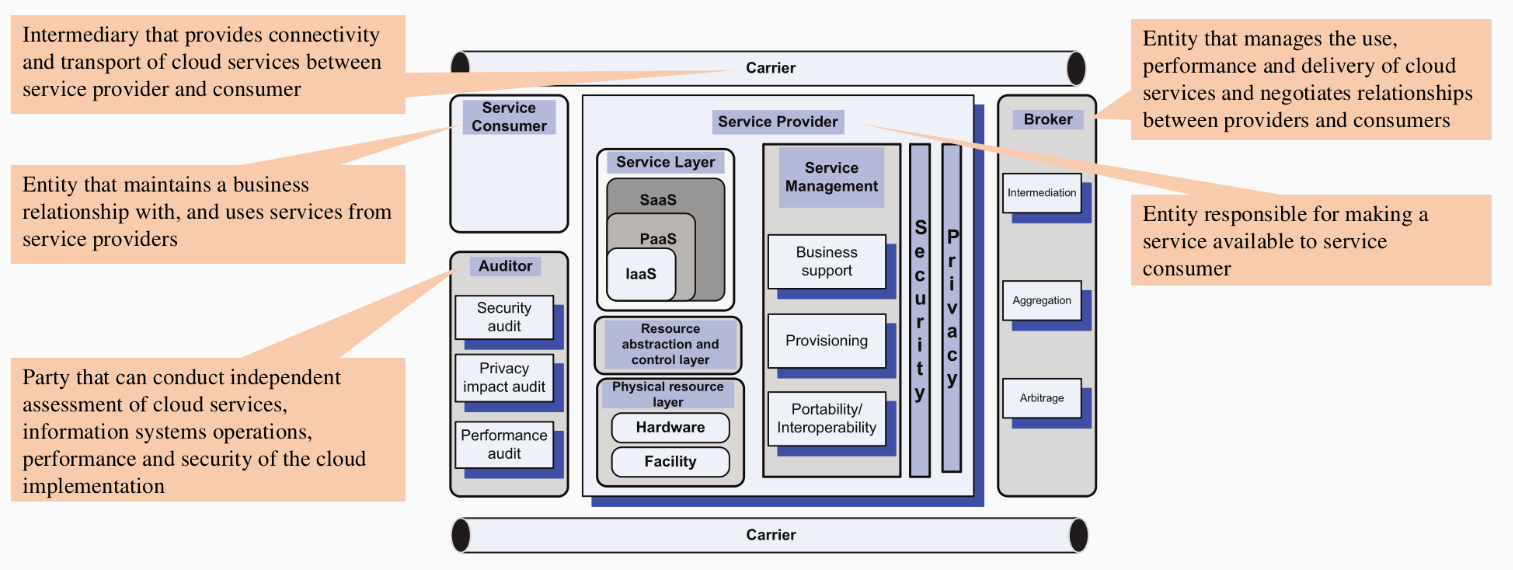
\includegraphics[scale=0.25]{images/cloudcomputingmodel.png}
    \caption{The NIST reference model for Cloud Computing}
    \label{fig:cloudmodel1}
\end{figure}
The NIST reference model for Cloud Computing is explained in figure \ref{fig:cloudmodel1}.

We spoke about \textbf{virtualisation} but what this term mean?
Virtualisation is the technique that abstract the computer resources, basically it isolate the hardware from the software and it make it possible to run different OS in the same infrastructure (like VirtualBox\footnote{An Oracle software for virtualisation and VM} for example). Let's see the difference between a Single and \textbf{Multi tenancy}:
In single tenancy each customer has its own software instance and requires a dedicated set of resources to fulfill the need of a customer. In a multy-tenancy environment instead of a single software instance a single instance of software runs on a server and serve multiple tenants, the resources management and costs are shared among tenants. With multi-tenancy you control a specific service without owning!

Another main feature of Cloud Computing is the \textbf{elasticity}, it means the ability to add or remove resources matching the workloads much more closely, it reduces the risk of overprovisioning and underprovisioning (we cancel idle time and the traffic overload). The risk of uderprovisioning is called \underline{transference of risk} we want to avoid that beacuse if users find that our service are unreachable there's the possibility of losing them (it happend in the past). In the other case, if we overprovision we pay for something that we don't use. The figure \ref{fig:elastic} is an example of the elasticity.
\begin{figure}
    \centering
    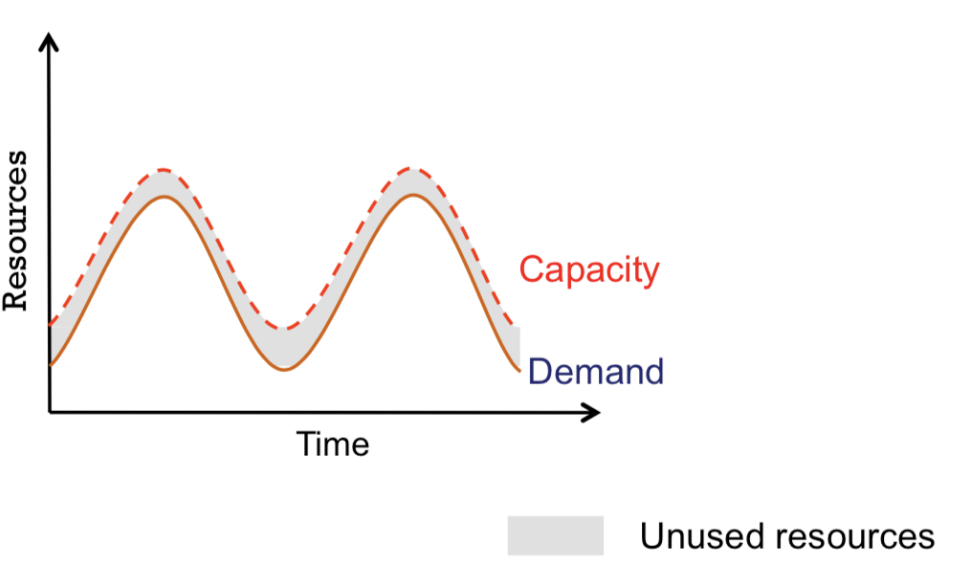
\includegraphics[scale=0.25]{images/elasticity.png}
    \caption{Example of elastic behaviour}
    \label{fig:elastic}
\end{figure}
\subsection{Cloud deployment models and delivery models}
The \textbf{deployment model} represent a specific type of cloud environment, distinguished by ownership, size and access
\begin{itemize}
    \item \textbf{Public} cloud: Are the providers like Google Microsoft or Amazon, their customers are the general public or a large industry group. They sell cloud services and manage the infrastructure. They are, of course, multi-tenancy
    \item \textbf{Private} cloud: It's for an exlusive use of an organisation, the infrastructure is located in the organisation or another party and it can decide if remotely host or not data
    \item \textbf{Community} cloud: It's for research community, is very similar to the Private cloud model
    \item \textbf{Hybrid} cloud: a mix of two or three model
\end{itemize}
The \textbf{Delivery models} define what "type" of service is offered, we have 3 big group
\begin{itemize}
    \item \textbf{Software-as-a-Service (SaaS):} These are the services like Netflix, Gmail. The user does not manage or control the infrastucture or the individual application (see figure \ref{fig:XaaS}), he only use the application to do things, this solution isn't good forreal-time applications.
    \item \textbf{Platform-as-a-Service (PaaS):} Allows a cloud user to deploy applications using programming languages and tools supported by the service provider. The user control the application but not the infrastructure under it (see figure \ref{fig:XaaS}).
    \item \textbf{Infrastructure-as-a-Service (IaaS):} With infrastructure we mean resources (like CPU, storage..), the user is able to deploy arbitrary software like OS and applications (see figure \ref{fig:XaaS}). IaaS exaples are server hosting, computing hardware, virtual instance (an example is EC2 from AWS)
    \item Others: like Hardware-as-a-Service, Database-as-a-Service (X-as-a-Service)
\end{itemize}
\begin{figure}[h]
    \centering
    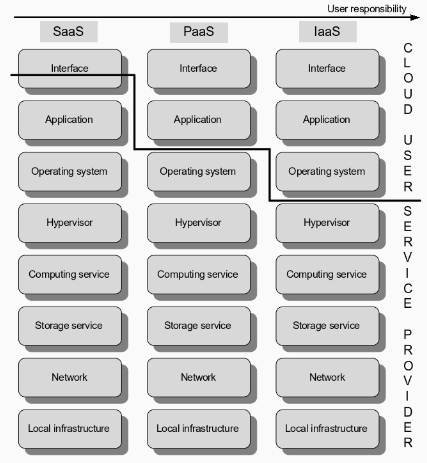
\includegraphics[scale=0.3]{images/XaaS.png}
    \caption{User control of the infrastructure}
    \label{fig:XaaS}
\end{figure}
\subsection{The market of cloud/fog solutions}
Speaking about real solution we can find three big OTT\footnote{Over The Top: the big company of computing}: Amazon which is a pioneer in IaaS (EC2 ecc.), Google which their efforts are focused in SaaS and Paas and Microsoft which its main involvement started with PaaS. Besides these big companies the market offers Open-source solution like OpenStack, OpenNebula ecc. In the first time the most of the revenue of cloud computing was generated by IaaS solutions and the market leader was AWS (and the same is nowadays). Amazon offers cloud services through a network of data centers on several continents, the regions do not share resurces and communicate through the Internet. When we buy an instance in practical we buy a virtual server with a well specified set of resources (CPU, storage ecc..). The user can choose the region where the virtual server should be placed and the instance type. When lauched the instance has a private IP address and a public one. In this process AWS get the request from the user, retrives a disk image of a VM and setup and locate the instance, last but not least give a IP address (through DHCP) and a MAC address. The user can interact using a Management Console, the SDK or using REST\footnote{Use HTTP request to communicate with the instance} requests.
